\subsection{Cross-entropy measure}

Let $\mathcal{X}$ be some sample space, and let $\mathcal{Y}$ be the label space $\{-1,1\}$, and assume that we want to learn the distribution of the labels $y$ conditioned on the value of a sample $x$, that is we want to learn the conditional probability $P(y|x)$ for $y \in {-1,1}$ and all $x\in \mathcal{X}$. Also, assume that the distribution $P(y|x)$ can be parametrized by choosing $w$ in some parameter space $\mathcal{W}$. That is, by choosing $w \in \mathcal{W}$ we get the value of $P_w(y|x)$ for $y \in {-1,1}$ and all $x\in \mathcal{X}$. In this context, the learning problem becomes to come up with a method for choosing some parameter $\hat{w} \in \mathcal{W}$ and hereby a corresponding distribution $P_{\hat{w}}(y|x)$, which somehow is our best guess of the true distribution of $y$ conditioned on $x$. The information we have available to base this choice on is some finite, labeled sample $S = \{(x_1,y_1),...,(x_N,y_N)\}$, where each $y_i$ is assumed to have been sampled from $P_w(y|x_i)$ and all of them independently from each other.

The maximum likelihood method for choosing $\hat{w}$ solves this problem by defining the likelihood function $L_S$ for the given sample $S$ as
\begin{align}
L_S(w) = \prod_{(x_n,y_n)\in \mathcal{S}}  P_w(y_n|x_n)
= \prod_{n=1}^N P_w(y_n|x_n)
\end{align}
and then saying that we should choose $\hat{w} \in \mathcal{W}$ such that $L_\mathcal{S}$ is maximized.

Since the function $-\ln$ is monotonically decreasing, this strategy is equivalent\footnote{I define two strategies to be equivalent, if and only if they end up choosing the same $\hat{w}$ for all possible samples $S = \{(x_1,y_1),...,(x_N,y_N)\}$.} to choosing $\hat{w} \in \mathcal{W}$ such that the function
\begin{align}
f_S(w) = -\ln \left( \prod_{n=1}^N P_w(y_n|x_n) \right) = \sum_{n=1}^N \left( - \ln P_w(y_n|x_n) \right)
\end{align}
is minimized. 

Since $y \in \{-1,1\}$, then we can write $P_w(y|x)$ as
\begin{align}
P_w(y|x)  = \\ 
[[y = 1]] P_w(y = 1|x) + [[y = 1]] P_w(y = -1|x) = \\ 
[[y = 1]] h_w(x) + [[y = 1]] (1 - h_w(x))
\end{align}
where we simply have defined $h_w(x) = P(y = 1 | x)$. We therefore have that
\begin{align}
- \ln P_w(y_n|x_n) = \\ 
-\ln ([[y = 1]] h_w(x) + [[y = -1]] (1 - h_w(x))) = \\ 
[[y = 1]](-\ln (h_w(x)) + [[y = -1]](-\ln (1 - h_w(x))) = \\ 
[[y = 1]]\left(\ln \left( \frac{1}{h_w(x)}\right)\right) + [[y = -1]]\left(\ln \left( \frac{1}{1 - h_w(x)}\right)\right)
\end{align}

By line (2) and line (6-9), we now get that
\begin{align}
f_S(w) = \sum_{n=1}^N \left[ [[y_n = 1]]\left(\ln \left( \frac{1}{h_w(x_n)}\right)\right) + [[y_n = -1]]\left(\ln \left( \frac{1}{1 - h_w(x_n)}\right)\right) \right]
\end{align}
As I have already said, we will end up with the same $\hat{w}$ for a given sample $S$, if we minimize $f_S(w)$ as if we maximize $L_S(w)$. If we had started by saying that we would like to estimate the probability $h_w(x) = P_w(y = 1|x)$ by choosing $\hat{w}$ such that we minimize the error function $f_S(w)$ defined as in line (10), we would have ended up with the same estimates of $P(y|x)$ for $y \in \{-1,1\}$ and $x\in \mathcal{X}$, as if we have used the maximum likelihood method. These two strategies are therefore equivalent.

If we now focus on logistic regression and set $h_w(x) = \Theta(w^T x) = \frac{e^{w^Tx}}{1 + e^{w^Tx}}$, we know from the book that $1 - h_w(x) = h_w(-x)$, which means that
\begin{align}
f_S(w) = \sum_{n=1}^N \left[ [[y_n = 1]]\left(\ln \left( \frac{1}{h_w(x_n)}\right)\right) + [[y_n = -1]]\left(\ln \left( \frac{1}{h_w(-x_n)}\right)\right) \right] = \\
 \sum_{n=1}^N  \ln \left( \frac{1}{h_w(y_nx_n)}\right)  = \sum_{n=1}^N  \ln \left( \frac{1}{\frac{e^{y_nw^Tx}}{1 + e^{y_ nw^Tx}}}\right)  = \sum_{n=1}^N  \ln \left( \frac{1 + e^{y_ nw^Tx}}{e^{y_ nw^Tx}}\right)  = \\
 \sum_{n=1}^N  \ln \left( 1 +e^{-y_ nw^Tx}\right)
\end{align}
Minimizing this function gives the same $w$ as minimizing:
\begin{align}
\frac{1}{N}f_S(w) = \frac{1}{N} \sum_{n=1}^N  \ln \left( 1 +e^{-y_ nw^Tx}\right)
\end{align}
This is exactly the function that the book says in statement (3.9) that we should minimize, when we search for the weights in logistic regression.

\subsection{Logistic regression loss gradient}

In the algorithm for logistic regression, we determine the parameter $w \in \mathbb{R}^m$ in our final hypothesis
\begin{align}
h_w(x) = P_w(y = 1|x) = \frac{e^{w^Tx}}{1 + e^{w^Tx}}
\end{align}
using a given labeled sample $S = \{(x_1,y_1),...,(x_N,y_N)\}$ by minizing the function
\begin{align}
E_{in}(w) = \frac{1}{N} \sum_{n=1}^N \ln(1 + e^{-y_n w^T x_n})
\end{align}
We use gradient descent to do this, which means we have to find the loss gradient $\nabla E_{in}(w)$. We can use matrix calculus to to differentiate $E_{in}$
\begin{align}
D_w (E_{in}(w)) = D_w\left( \frac{1}{N} \sum_{n=1}^N \ln(1 + e^{-y_n w^T x_n}) \right) = \\ 
 \frac{1}{N} \sum_{n=1}^N D_w \left( \ln(1 + e^{-y_n w^T x_n}) \right). 
\end{align}
Let us now focus on the inside of the sum
\begin{align}
D_w \left( \ln(1 + e^{-y_n w^T x_n}) \right) = \frac{D_w ( 1 + e^{-y_n w^T x_n})}{1 + e^{-y_n w^T x_n}} = \\ 
\frac{D_w (e^{-y_n w^T x_n})}{1 + e^{-y_n w^T x_n}} =
\frac{e^{-y_n w^T x_n} D_w(-y_nw^Tx)}{1 + e^{-y_n w^T x_n}} = \\ 
-y_n x_n \frac{e^{-y_n w^T x_n}}{1 + e^{-y_n w^T x_n}} = -y_n x_n \Theta(-y_n w^T x_n)
\end{align}
Line (13-14) and line (15-17) now gives us that
\begin{align}
D_w (E_{in}(w)) =  \frac{1}{N} \sum_{n=1}^N D_w \left( \ln(1 + e^{-y_n w^T x_n}) \right) =
\frac{1}{N} \sum_{n=1}^N  -y_n x_n \Theta(-y_n w^T x_n) 
\end{align}
which is what the exercise asked us to show. 

\subsection{Logistic regression implementation}

My implementation is written in python with the use of the scipy library. It has a little more code than strictly necessary for two reasons. First, I have experimented with the book's proposal of using a combination of the norm of the gradient and the training error made by the classifier resulting from the weigths in the given iteration as a stopping criterion for the algorithm. This means that I have to construct the classifier from the weights and calculate the resulting error on the training set in each iteration of the algorithm. Second, I log information from each iteration in order to be able to investigate how the algorithm evolves through time. 

As input, my main function $log\_reg$ takes a scipy 2d-array as x (the sample) and a scipy 1d-array as y (the labels). Additionally, the user can specify some more arguments to control the hyper-parameters of the algorithm. As output, the function returns a dictionary with the weights found by the algorithm, the classifier given by these weigths and some arrays that log the history of different, interesting variables through the iterations of the algorithm. Here is my source code:
\begin{Verbatim}[fontsize = \relsize{-2}]
import scipy as scp
import scipy.linalg as lalg
----------------------------------------------------------------------------------
def log_reg(x, y, rate = 1, gnorm_stop = 0.01, error_stop = 0.05,
            iterations_stop = 1000000, start_weigths = None, seed = 1989) :
    
    scp.random.seed(seed)
    if (start_weigths == None) : w = scp.random.normal(size = x.shape[1])
    else : w = start_weights
    
    n = x.shape[0]; ws = []; gnorms = []; es = []; i = 1
    
    while (i <= iterations_stop) : 
    
        ws.append(w)
        g = gradient(x, y, w, n); gnorm = lalg.norm(g); gnorms.append(gnorm)
        c = make_classifier(w); e = error(x,y,c,n); es.append(e)
        
        if terminate(e, error_stop, gnorm, gnorm_stop) : break
        
        w = w + (-g) * rate; i = i + 1
    
    return {'classifier' : c, 'weights' : w, 'gnorm_history' : scp.array(gnorms), 
            'weight_history' : scp.array(ws), 'error_history' : scp.array(es)}
----------------------------------------------------------------------------------
def gradient(x, y, w, n) :
    num = x * y[:,scp.newaxis]
    den = scp.dot(x, w) * y
    den = scp.exp(den) + 1
    quotient = num / den[:,scp.newaxis]
    avg = scp.sum(quotient, axis = 0) / n
    return - avg
----------------------------------------------------------------------------------
def make_classifier(w) :
    def classifier(x) :
        p = scp.exp(scp.dot(x,w))/(1 + scp.exp(scp.dot(x,w)))
        if (p > 0.5) : return 1
        else : return -1
    return classifier
----------------------------------------------------------------------------------
def error(x, y, classifier, n) :
    pred = scp.apply_along_axis(classifier, 1, x)
    e = abs((pred - y)) / 2
    e = scp.sum(e) / n
    return e
----------------------------------------------------------------------------------
def terminate(e, error_stop, gnorm, gnorm_stop) :
    if ((gnorm < gnorm_stop) and (e < error_stop )) : return True
    else : return False
----------------------------------------------------------------------------------
\end{Verbatim}

\subsection{Iris Flower Data}

As I mentioned in the last section, I have experimented with using both the norm of the gradient and size of the training error as the stopping criterion of my algorithm. Specifically, I have said that the algorithm should stop iterating, when the norm of the gradient is less than 0.01, and the training error - calculated as the fraction of wrongly classified points - is less than 0.05. If this criterion has not been fulfilled after the $1000000^{th}$ iteration, the algorithm should also stop. These hyper parameters can be changed by specifying arguments to my function. If no other start weights are specified, then my implementation samples to start weights from a standard normal distribution. Here is a plot showing how the values of the weights develop through the iterations of the algorithm:
\begin{center}
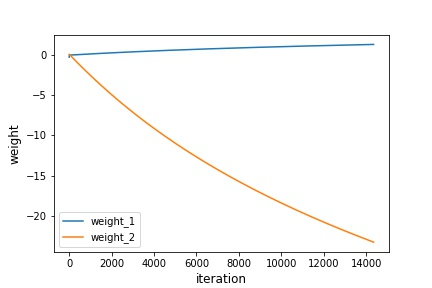
\includegraphics[scale = 0.5]{logistic_regression/weightplot3.jpg}
\end{center}
When we look at this plot, it does not look like the value of the weights have converged, when the algorithm stopped. Here are two plots of the norm of gradient through the iterations, where I have cut away the 10 first iterations in the second plot:
\begin{center}
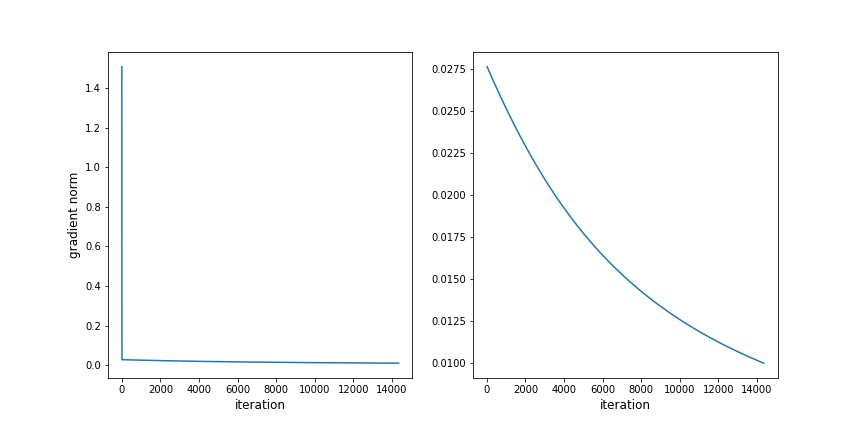
\includegraphics[scale = 0.4]{logistic_regression/normplot1.jpg}
\end{center}
Here, we also see from the second plot that the norm of the gradient is still in the process of getting even smaller, when the algorithm stops. When we look at the plot of the development of the training error through the iterations, we see something different:
\begin{center}
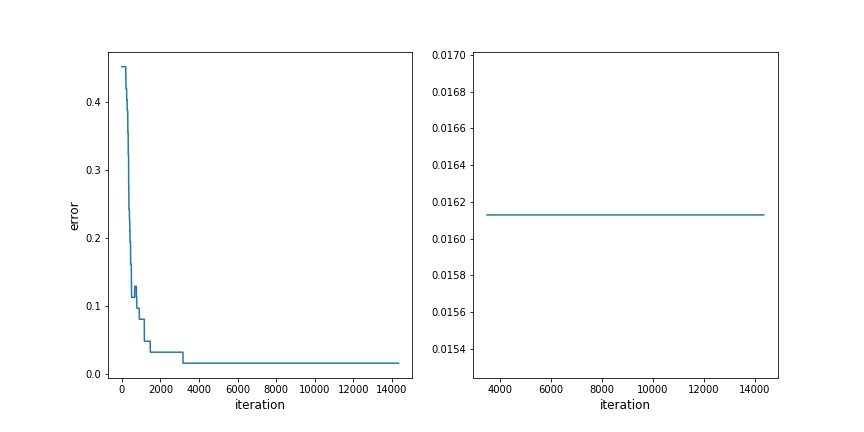
\includegraphics[scale=0.4]{logistic_regression/errorplot.jpg}
\end{center}
After around iteration number 3500, the training error does not improve, but is constant with the value of 0.0161. This corresponds to 1 of 62 training examples being wrongly classified. In terms of only getting a low training error, the majority of the iterations are therefore wasted. On the hand, if we wanted to get our weights as close as possible to the weights maximizing the likelihood of the data in the model space of logistic regression, then we should have continued the iterations, since the weights have not converged yet.

All in all, my implementation of logistic regression with the chosen hyper-parameters end up giving me the weights $(1.31, -23.28)$. The classifier constructed from these weights gives me a test error of 0.038. This corresponds to 1 of the 26 test examples being wrongly classified.
